\documentclass[twoside]{book}

% Packages required by doxygen
\usepackage{fixltx2e}
\usepackage{calc}
\usepackage{doxygen}
\usepackage[export]{adjustbox} % also loads graphicx
\usepackage{graphicx}
\usepackage[utf8]{inputenc}
\usepackage{makeidx}
\usepackage{multicol}
\usepackage{multirow}
\PassOptionsToPackage{warn}{textcomp}
\usepackage{textcomp}
\usepackage[nointegrals]{wasysym}
\usepackage[table]{xcolor}

% Font selection
\usepackage[T1]{fontenc}
\usepackage[scaled=.90]{helvet}
\usepackage{courier}
\usepackage{amssymb}
\usepackage{sectsty}
\renewcommand{\familydefault}{\sfdefault}
\allsectionsfont{%
  \fontseries{bc}\selectfont%
  \color{darkgray}%
}
\renewcommand{\DoxyLabelFont}{%
  \fontseries{bc}\selectfont%
  \color{darkgray}%
}
\newcommand{\+}{\discretionary{\mbox{\scriptsize$\hookleftarrow$}}{}{}}

% Page & text layout
\usepackage{geometry}
\geometry{%
  a4paper,%
  top=2.5cm,%
  bottom=2.5cm,%
  left=2.5cm,%
  right=2.5cm%
}
\tolerance=750
\hfuzz=15pt
\hbadness=750
\setlength{\emergencystretch}{15pt}
\setlength{\parindent}{0cm}
\setlength{\parskip}{3ex plus 2ex minus 2ex}
\makeatletter
\renewcommand{\paragraph}{%
  \@startsection{paragraph}{4}{0ex}{-1.0ex}{1.0ex}{%
    \normalfont\normalsize\bfseries\SS@parafont%
  }%
}
\renewcommand{\subparagraph}{%
  \@startsection{subparagraph}{5}{0ex}{-1.0ex}{1.0ex}{%
    \normalfont\normalsize\bfseries\SS@subparafont%
  }%
}
\makeatother

% Headers & footers
\usepackage{fancyhdr}
\pagestyle{fancyplain}
\fancyhead[LE]{\fancyplain{}{\bfseries\thepage}}
\fancyhead[CE]{\fancyplain{}{}}
\fancyhead[RE]{\fancyplain{}{\bfseries\leftmark}}
\fancyhead[LO]{\fancyplain{}{\bfseries\rightmark}}
\fancyhead[CO]{\fancyplain{}{}}
\fancyhead[RO]{\fancyplain{}{\bfseries\thepage}}
\fancyfoot[LE]{\fancyplain{}{}}
\fancyfoot[CE]{\fancyplain{}{}}
\fancyfoot[RE]{\fancyplain{}{\bfseries\scriptsize Generated by Doxygen }}
\fancyfoot[LO]{\fancyplain{}{\bfseries\scriptsize Generated by Doxygen }}
\fancyfoot[CO]{\fancyplain{}{}}
\fancyfoot[RO]{\fancyplain{}{}}
\renewcommand{\footrulewidth}{0.4pt}
\renewcommand{\chaptermark}[1]{%
  \markboth{#1}{}%
}
\renewcommand{\sectionmark}[1]{%
  \markright{\thesection\ #1}%
}

% Indices & bibliography
\usepackage{natbib}
\usepackage[titles]{tocloft}
\setcounter{tocdepth}{3}
\setcounter{secnumdepth}{5}
\makeindex

% Hyperlinks (required, but should be loaded last)
\usepackage{ifpdf}
\ifpdf
  \usepackage[pdftex,pagebackref=true]{hyperref}
\else
  \usepackage[ps2pdf,pagebackref=true]{hyperref}
\fi
\hypersetup{%
  colorlinks=true,%
  linkcolor=blue,%
  citecolor=blue,%
  unicode%
}

% Custom commands
\newcommand{\clearemptydoublepage}{%
  \newpage{\pagestyle{empty}\cleardoublepage}%
}

\usepackage{caption}
\captionsetup{labelsep=space,justification=centering,font={bf},singlelinecheck=off,skip=4pt,position=top}

%===== C O N T E N T S =====

\begin{document}

% Titlepage & ToC
\hypersetup{pageanchor=false,
             bookmarksnumbered=true,
             pdfencoding=unicode
            }
\pagenumbering{roman}
\begin{titlepage}
\vspace*{7cm}
\begin{center}%
{\Large S\+O\+P\+ER Practica 2 }\\
\vspace*{1cm}
{\large Generated by Doxygen 1.8.11}\\
\end{center}
\end{titlepage}
\clearemptydoublepage
\tableofcontents
\clearemptydoublepage
\pagenumbering{arabic}
\hypersetup{pageanchor=true}

%--- Begin generated contents ---
\chapter{File Index}
\section{File List}
Here is a list of all documented files with brief descriptions\+:\begin{DoxyCompactList}
\item\contentsline{section}{\hyperlink{ejercicio2_8c}{ejercicio2.\+c} \\*Ejercicio2 Creación de 4 procesos hijos que duermen durante 30s mientras que el proceso padre espera 5s y después envía a cada proceso hijo la señal de finalización S\+I\+G\+T\+E\+RM }{\pageref{ejercicio2_8c}}{}
\item\contentsline{section}{\hyperlink{ejercicio4_8c}{ejercicio4.\+c} \\*Ejercicio4 Manejo de señales entre procesos hijos y padre }{\pageref{ejercicio4_8c}}{}
\item\contentsline{section}{\hyperlink{ejercicio6a_8c}{ejercicio6a.\+c} \\*Ejercicio6a Toma de contacto con la funcion alarm() }{\pageref{ejercicio6a_8c}}{}
\item\contentsline{section}{\hyperlink{ejercicio6b_8c}{ejercicio6b.\+c} \\*Ejercicio6b Toma de contacto con la funcion sigfillset() }{\pageref{ejercicio6b_8c}}{}
\item\contentsline{section}{\hyperlink{semaforos_8c}{semaforos.\+c} \\*Ejercicio9 }{\pageref{semaforos_8c}}{}
\item\contentsline{section}{\hyperlink{semaforos_8h}{semaforos.\+h} \\*Utilidades de manejo de semaforos }{\pageref{semaforos_8h}}{}
\end{DoxyCompactList}

\chapter{File Documentation}
\hypertarget{ejercicio2_8c}{}\section{ejercicio2.\+c File Reference}
\label{ejercicio2_8c}\index{ejercicio2.\+c@{ejercicio2.\+c}}


Ejercicio2 Creación de 4 procesos hijos que duermen durante 30s mientras que el proceso padre espera 5s y después envía a cada proceso hijo la señal de finalización S\+I\+G\+T\+E\+RM.  


{\ttfamily \#include $<$stdio.\+h$>$}\\*
{\ttfamily \#include $<$stdlib.\+h$>$}\\*
{\ttfamily \#include $<$string.\+h$>$}\\*
{\ttfamily \#include $<$sys/types.\+h$>$}\\*
{\ttfamily \#include $<$sys/wait.\+h$>$}\\*
{\ttfamily \#include $<$unistd.\+h$>$}\\*
{\ttfamily \#include $<$errno.\+h$>$}\\*
{\ttfamily \#include $<$signal.\+h$>$}\\*
Include dependency graph for ejercicio2.\+c\+:
\nopagebreak
\begin{figure}[H]
\begin{center}
\leavevmode
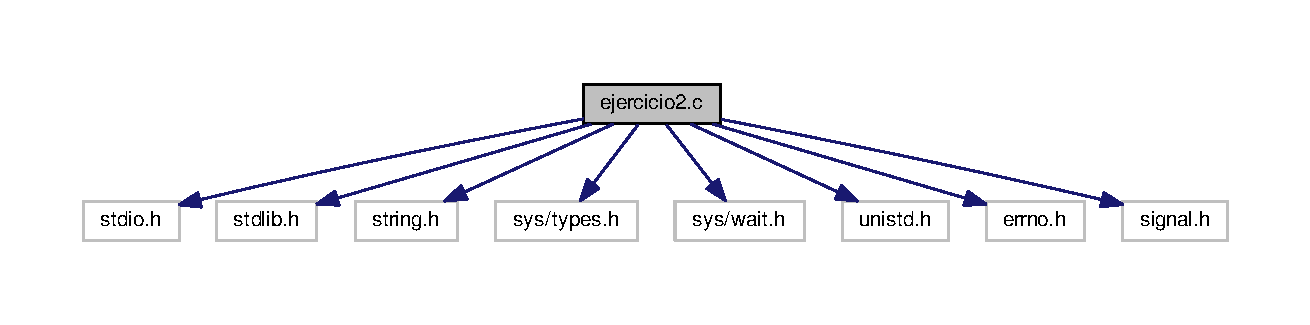
\includegraphics[width=350pt]{ejercicio2_8c__incl}
\end{center}
\end{figure}
\subsection*{Macros}
\begin{DoxyCompactItemize}
\item 
\#define \hyperlink{ejercicio2_8c_a469b1ab8d3ecbd62178c442e0d19c200}{N\+\_\+\+C\+H\+I\+L\+DS}~4
\end{DoxyCompactItemize}
\subsection*{Functions}
\begin{DoxyCompactItemize}
\item 
int {\bfseries main} ()\hypertarget{ejercicio2_8c_ae66f6b31b5ad750f1fe042a706a4e3d4}{}\label{ejercicio2_8c_ae66f6b31b5ad750f1fe042a706a4e3d4}

\end{DoxyCompactItemize}


\subsection{Detailed Description}
Ejercicio2 Creación de 4 procesos hijos que duermen durante 30s mientras que el proceso padre espera 5s y después envía a cada proceso hijo la señal de finalización S\+I\+G\+T\+E\+RM. 

\begin{DoxyAuthor}{Author}
Alejandro Santorum \& David Cabornero (G2202-\/\+Pareja7) 
\end{DoxyAuthor}
\begin{DoxyVersion}{Version}
1.\+0 
\end{DoxyVersion}
\begin{DoxyDate}{Date}
31-\/03-\/2018 
\end{DoxyDate}


\subsection{Macro Definition Documentation}
\index{ejercicio2.\+c@{ejercicio2.\+c}!N\+\_\+\+C\+H\+I\+L\+DS@{N\+\_\+\+C\+H\+I\+L\+DS}}
\index{N\+\_\+\+C\+H\+I\+L\+DS@{N\+\_\+\+C\+H\+I\+L\+DS}!ejercicio2.\+c@{ejercicio2.\+c}}
\subsubsection[{\texorpdfstring{N\+\_\+\+C\+H\+I\+L\+DS}{N_CHILDS}}]{\setlength{\rightskip}{0pt plus 5cm}\#define N\+\_\+\+C\+H\+I\+L\+DS~4}\hypertarget{ejercicio2_8c_a469b1ab8d3ecbd62178c442e0d19c200}{}\label{ejercicio2_8c_a469b1ab8d3ecbd62178c442e0d19c200}
Número de procesos hijos 
\hypertarget{ejercicio4_8c}{}\section{ejercicio4.\+c File Reference}
\label{ejercicio4_8c}\index{ejercicio4.\+c@{ejercicio4.\+c}}


Ejercicio4 Manejo de señales entre procesos hijos y padre.  


{\ttfamily \#include $<$stdio.\+h$>$}\\*
{\ttfamily \#include $<$stdlib.\+h$>$}\\*
{\ttfamily \#include $<$string.\+h$>$}\\*
{\ttfamily \#include $<$sys/types.\+h$>$}\\*
{\ttfamily \#include $<$sys/wait.\+h$>$}\\*
{\ttfamily \#include $<$unistd.\+h$>$}\\*
{\ttfamily \#include $<$errno.\+h$>$}\\*
{\ttfamily \#include $<$signal.\+h$>$}\\*
{\ttfamily \#include $<$ctype.\+h$>$}\\*
Include dependency graph for ejercicio4.\+c\+:
\nopagebreak
\begin{figure}[H]
\begin{center}
\leavevmode
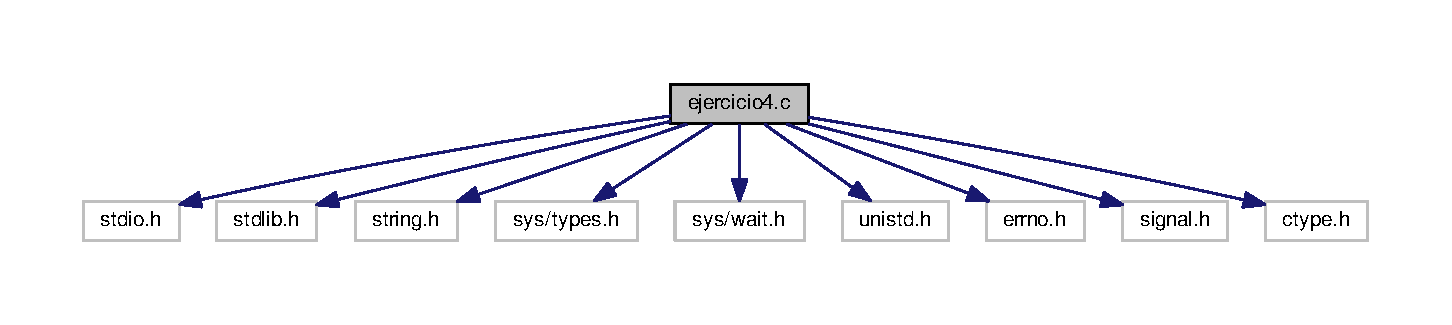
\includegraphics[width=350pt]{ejercicio4_8c__incl}
\end{center}
\end{figure}
\subsection*{Macros}
\begin{DoxyCompactItemize}
\item 
\#define \hyperlink{ejercicio4_8c_a1eae4448563ec6ad91f74fc8e8ba228d}{N\+\_\+\+P\+R\+I\+NT}~10
\end{DoxyCompactItemize}
\subsection*{Functions}
\begin{DoxyCompactItemize}
\item 
int \hyperlink{ejercicio4_8c_a86a4f2b7e18ef771ecf42d7aca5c9fde}{is\+\_\+valid\+\_\+integer} (char $\ast$input)
\begin{DoxyCompactList}\small\item\em evalua si un argumento de entrada es verdaderamente un entero \end{DoxyCompactList}\item 
void \hyperlink{ejercicio4_8c_affae6eb1392c68ed64ab02cd348429d2}{handler\+\_\+\+S\+I\+G\+U\+S\+R1} (int sig)
\begin{DoxyCompactList}\small\item\em nuevo manejador de la señal S\+I\+G\+U\+S\+R1. Su funcionalidad es simplemente no hacer nada. \end{DoxyCompactList}\item 
int {\bfseries main} (int argc, char $\ast$argv\mbox{[}$\,$\mbox{]})\hypertarget{ejercicio4_8c_a0ddf1224851353fc92bfbff6f499fa97}{}\label{ejercicio4_8c_a0ddf1224851353fc92bfbff6f499fa97}

\end{DoxyCompactItemize}


\subsection{Detailed Description}
Ejercicio4 Manejo de señales entre procesos hijos y padre. 

\begin{DoxyAuthor}{Author}
Alejandro Santorum \& David Cabornero (G2202-\/\+Pareja7) 
\end{DoxyAuthor}
\begin{DoxyVersion}{Version}
1.\+0 
\end{DoxyVersion}
\begin{DoxyDate}{Date}
31-\/03-\/2018 
\end{DoxyDate}


\subsection{Macro Definition Documentation}
\index{ejercicio4.\+c@{ejercicio4.\+c}!N\+\_\+\+P\+R\+I\+NT@{N\+\_\+\+P\+R\+I\+NT}}
\index{N\+\_\+\+P\+R\+I\+NT@{N\+\_\+\+P\+R\+I\+NT}!ejercicio4.\+c@{ejercicio4.\+c}}
\subsubsection[{\texorpdfstring{N\+\_\+\+P\+R\+I\+NT}{N_PRINT}}]{\setlength{\rightskip}{0pt plus 5cm}\#define N\+\_\+\+P\+R\+I\+NT~10}\hypertarget{ejercicio4_8c_a1eae4448563ec6ad91f74fc8e8ba228d}{}\label{ejercicio4_8c_a1eae4448563ec6ad91f74fc8e8ba228d}
Número de impresiones por pantalla de cada hijo 

\subsection{Function Documentation}
\index{ejercicio4.\+c@{ejercicio4.\+c}!handler\+\_\+\+S\+I\+G\+U\+S\+R1@{handler\+\_\+\+S\+I\+G\+U\+S\+R1}}
\index{handler\+\_\+\+S\+I\+G\+U\+S\+R1@{handler\+\_\+\+S\+I\+G\+U\+S\+R1}!ejercicio4.\+c@{ejercicio4.\+c}}
\subsubsection[{\texorpdfstring{handler\+\_\+\+S\+I\+G\+U\+S\+R1(int sig)}{handler_SIGUSR1(int sig)}}]{\setlength{\rightskip}{0pt plus 5cm}void handler\+\_\+\+S\+I\+G\+U\+S\+R1 (
\begin{DoxyParamCaption}
\item[{int}]{sig}
\end{DoxyParamCaption}
)}\hypertarget{ejercicio4_8c_affae6eb1392c68ed64ab02cd348429d2}{}\label{ejercicio4_8c_affae6eb1392c68ed64ab02cd348429d2}


nuevo manejador de la señal S\+I\+G\+U\+S\+R1. Su funcionalidad es simplemente no hacer nada. 


\begin{DoxyParams}{Parameters}
{\em sig} & -\/ la señal que utilizará este manejador cuando sea llamada \\
\hline
\end{DoxyParams}
\begin{DoxyReturn}{Returns}
void. 
\end{DoxyReturn}
\index{ejercicio4.\+c@{ejercicio4.\+c}!is\+\_\+valid\+\_\+integer@{is\+\_\+valid\+\_\+integer}}
\index{is\+\_\+valid\+\_\+integer@{is\+\_\+valid\+\_\+integer}!ejercicio4.\+c@{ejercicio4.\+c}}
\subsubsection[{\texorpdfstring{is\+\_\+valid\+\_\+integer(char $\ast$input)}{is_valid_integer(char *input)}}]{\setlength{\rightskip}{0pt plus 5cm}int is\+\_\+valid\+\_\+integer (
\begin{DoxyParamCaption}
\item[{char $\ast$}]{input}
\end{DoxyParamCaption}
)}\hypertarget{ejercicio4_8c_a86a4f2b7e18ef771ecf42d7aca5c9fde}{}\label{ejercicio4_8c_a86a4f2b7e18ef771ecf42d7aca5c9fde}


evalua si un argumento de entrada es verdaderamente un entero 


\begin{DoxyParams}{Parameters}
{\em input} & -\/ contiene la cadena de caracteres sospechosa de ser un entero \\
\hline
\end{DoxyParams}
\begin{DoxyReturn}{Returns}
1 si es un entero, 0 en caso contrario. 
\end{DoxyReturn}

\hypertarget{ejercicio6a_8c}{}\section{ejercicio6a.\+c File Reference}
\label{ejercicio6a_8c}\index{ejercicio6a.\+c@{ejercicio6a.\+c}}


Ejercicio6a Toma de contacto con la funcion alarm()  


{\ttfamily \#include $<$stdio.\+h$>$}\\*
{\ttfamily \#include $<$stdlib.\+h$>$}\\*
{\ttfamily \#include $<$string.\+h$>$}\\*
{\ttfamily \#include $<$sys/types.\+h$>$}\\*
{\ttfamily \#include $<$sys/wait.\+h$>$}\\*
{\ttfamily \#include $<$unistd.\+h$>$}\\*
{\ttfamily \#include $<$errno.\+h$>$}\\*
{\ttfamily \#include $<$signal.\+h$>$}\\*
{\ttfamily \#include $<$ctype.\+h$>$}\\*
Include dependency graph for ejercicio6a.\+c\+:
\nopagebreak
\begin{figure}[H]
\begin{center}
\leavevmode
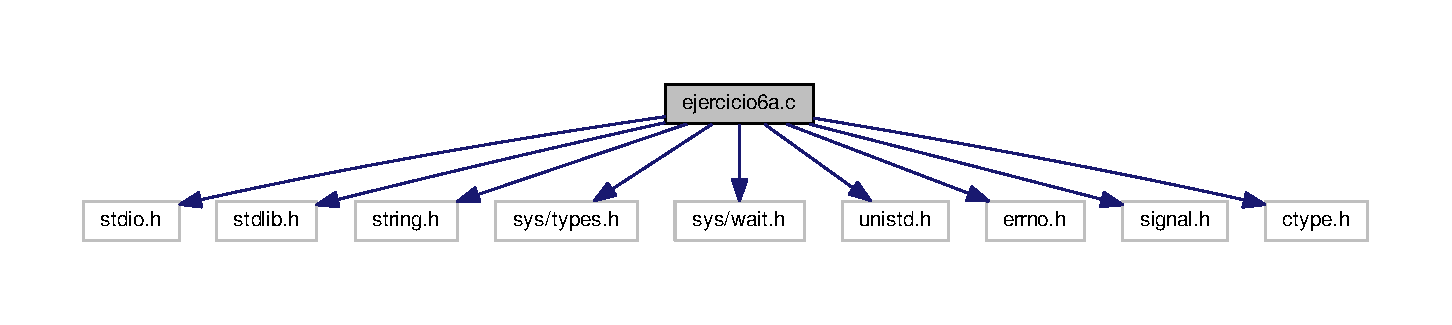
\includegraphics[width=350pt]{ejercicio6a_8c__incl}
\end{center}
\end{figure}
\subsection*{Macros}
\begin{DoxyCompactItemize}
\item 
\#define \hyperlink{ejercicio6a_8c_aaf0952059602752258dccaa015d7b54a}{N\+UM}~5
\end{DoxyCompactItemize}
\subsection*{Functions}
\begin{DoxyCompactItemize}
\item 
int {\bfseries main} (int argc, char $\ast$argv\mbox{[}$\,$\mbox{]})\hypertarget{ejercicio6a_8c_a0ddf1224851353fc92bfbff6f499fa97}{}\label{ejercicio6a_8c_a0ddf1224851353fc92bfbff6f499fa97}

\end{DoxyCompactItemize}


\subsection{Detailed Description}
Ejercicio6a Toma de contacto con la funcion alarm() 

\begin{DoxyAuthor}{Author}
Alejandro Santorum \& David Cabornero (G2202-\/\+Pareja7) 
\end{DoxyAuthor}
\begin{DoxyVersion}{Version}
1.\+0 
\end{DoxyVersion}
\begin{DoxyDate}{Date}
31-\/03-\/2018 
\end{DoxyDate}


\subsection{Macro Definition Documentation}
\index{ejercicio6a.\+c@{ejercicio6a.\+c}!N\+UM@{N\+UM}}
\index{N\+UM@{N\+UM}!ejercicio6a.\+c@{ejercicio6a.\+c}}
\subsubsection[{\texorpdfstring{N\+UM}{NUM}}]{\setlength{\rightskip}{0pt plus 5cm}\#define N\+UM~5}\hypertarget{ejercicio6a_8c_aaf0952059602752258dccaa015d7b54a}{}\label{ejercicio6a_8c_aaf0952059602752258dccaa015d7b54a}
Número de impresiones 
\hypertarget{ejercicio6b_8c}{}\section{ejercicio6b.\+c File Reference}
\label{ejercicio6b_8c}\index{ejercicio6b.\+c@{ejercicio6b.\+c}}


Ejercicio6b Toma de contacto con la funcion sigfillset()  


{\ttfamily \#include $<$stdio.\+h$>$}\\*
{\ttfamily \#include $<$stdlib.\+h$>$}\\*
{\ttfamily \#include $<$string.\+h$>$}\\*
{\ttfamily \#include $<$sys/types.\+h$>$}\\*
{\ttfamily \#include $<$sys/wait.\+h$>$}\\*
{\ttfamily \#include $<$unistd.\+h$>$}\\*
{\ttfamily \#include $<$errno.\+h$>$}\\*
{\ttfamily \#include $<$signal.\+h$>$}\\*
{\ttfamily \#include $<$ctype.\+h$>$}\\*
Include dependency graph for ejercicio6b.\+c\+:
\nopagebreak
\begin{figure}[H]
\begin{center}
\leavevmode
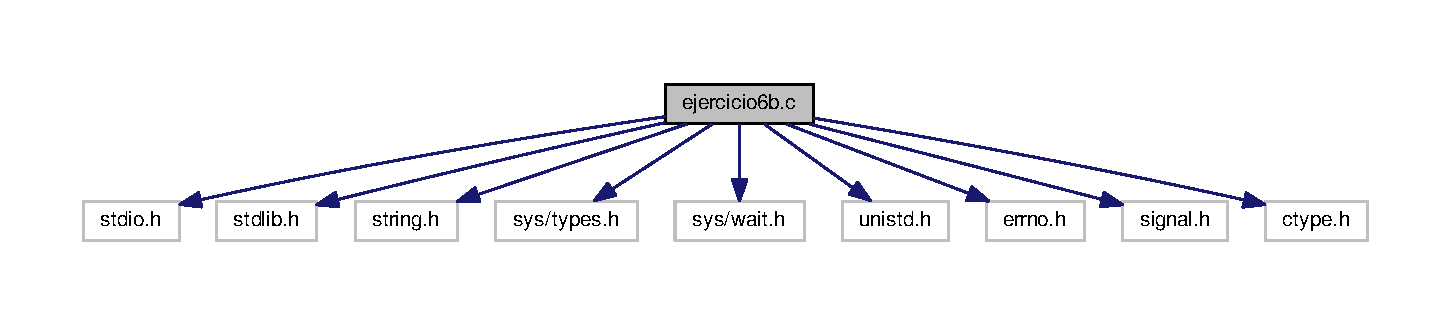
\includegraphics[width=350pt]{ejercicio6b_8c__incl}
\end{center}
\end{figure}
\subsection*{Macros}
\begin{DoxyCompactItemize}
\item 
\#define \hyperlink{ejercicio6b_8c_aaf0952059602752258dccaa015d7b54a}{N\+UM}~5
\end{DoxyCompactItemize}
\subsection*{Functions}
\begin{DoxyCompactItemize}
\item 
void \hyperlink{ejercicio6b_8c_aaf4e4635ab40745568d100c91f0d5a19}{handler\+\_\+\+S\+I\+G\+T\+E\+RM} (int sig)
\begin{DoxyCompactList}\small\item\em nuevo manejador de la señal S\+I\+G\+T\+E\+RM. Su funcionalidad es simplemente imprimir el P\+ID y un mensaje. \end{DoxyCompactList}\item 
int {\bfseries main} (int argc, char $\ast$argv\mbox{[}$\,$\mbox{]})\hypertarget{ejercicio6b_8c_a0ddf1224851353fc92bfbff6f499fa97}{}\label{ejercicio6b_8c_a0ddf1224851353fc92bfbff6f499fa97}

\end{DoxyCompactItemize}


\subsection{Detailed Description}
Ejercicio6b Toma de contacto con la funcion sigfillset() 

\begin{DoxyAuthor}{Author}
Alejandro Santorum \& David Cabornero (G2202-\/\+Pareja7) 
\end{DoxyAuthor}
\begin{DoxyVersion}{Version}
1.\+0 
\end{DoxyVersion}
\begin{DoxyDate}{Date}
31-\/03-\/2018 
\end{DoxyDate}


\subsection{Macro Definition Documentation}
\index{ejercicio6b.\+c@{ejercicio6b.\+c}!N\+UM@{N\+UM}}
\index{N\+UM@{N\+UM}!ejercicio6b.\+c@{ejercicio6b.\+c}}
\subsubsection[{\texorpdfstring{N\+UM}{NUM}}]{\setlength{\rightskip}{0pt plus 5cm}\#define N\+UM~5}\hypertarget{ejercicio6b_8c_aaf0952059602752258dccaa015d7b54a}{}\label{ejercicio6b_8c_aaf0952059602752258dccaa015d7b54a}
Número de impresiones 

\subsection{Function Documentation}
\index{ejercicio6b.\+c@{ejercicio6b.\+c}!handler\+\_\+\+S\+I\+G\+T\+E\+RM@{handler\+\_\+\+S\+I\+G\+T\+E\+RM}}
\index{handler\+\_\+\+S\+I\+G\+T\+E\+RM@{handler\+\_\+\+S\+I\+G\+T\+E\+RM}!ejercicio6b.\+c@{ejercicio6b.\+c}}
\subsubsection[{\texorpdfstring{handler\+\_\+\+S\+I\+G\+T\+E\+R\+M(int sig)}{handler_SIGTERM(int sig)}}]{\setlength{\rightskip}{0pt plus 5cm}void handler\+\_\+\+S\+I\+G\+T\+E\+RM (
\begin{DoxyParamCaption}
\item[{int}]{sig}
\end{DoxyParamCaption}
)}\hypertarget{ejercicio6b_8c_aaf4e4635ab40745568d100c91f0d5a19}{}\label{ejercicio6b_8c_aaf4e4635ab40745568d100c91f0d5a19}


nuevo manejador de la señal S\+I\+G\+T\+E\+RM. Su funcionalidad es simplemente imprimir el P\+ID y un mensaje. 


\begin{DoxyParams}{Parameters}
{\em sig} & -\/ la señal que utilizará este manejador cuando sea llamada \\
\hline
\end{DoxyParams}
\begin{DoxyReturn}{Returns}
void. 
\end{DoxyReturn}

\hypertarget{semaforos_8c}{}\section{semaforos.\+c File Reference}
\label{semaforos_8c}\index{semaforos.\+c@{semaforos.\+c}}


Ejercicio9.  


{\ttfamily \#include \char`\"{}semaforos.\+h\char`\"{}}\\*
Include dependency graph for semaforos.\+c\+:
\nopagebreak
\begin{figure}[H]
\begin{center}
\leavevmode
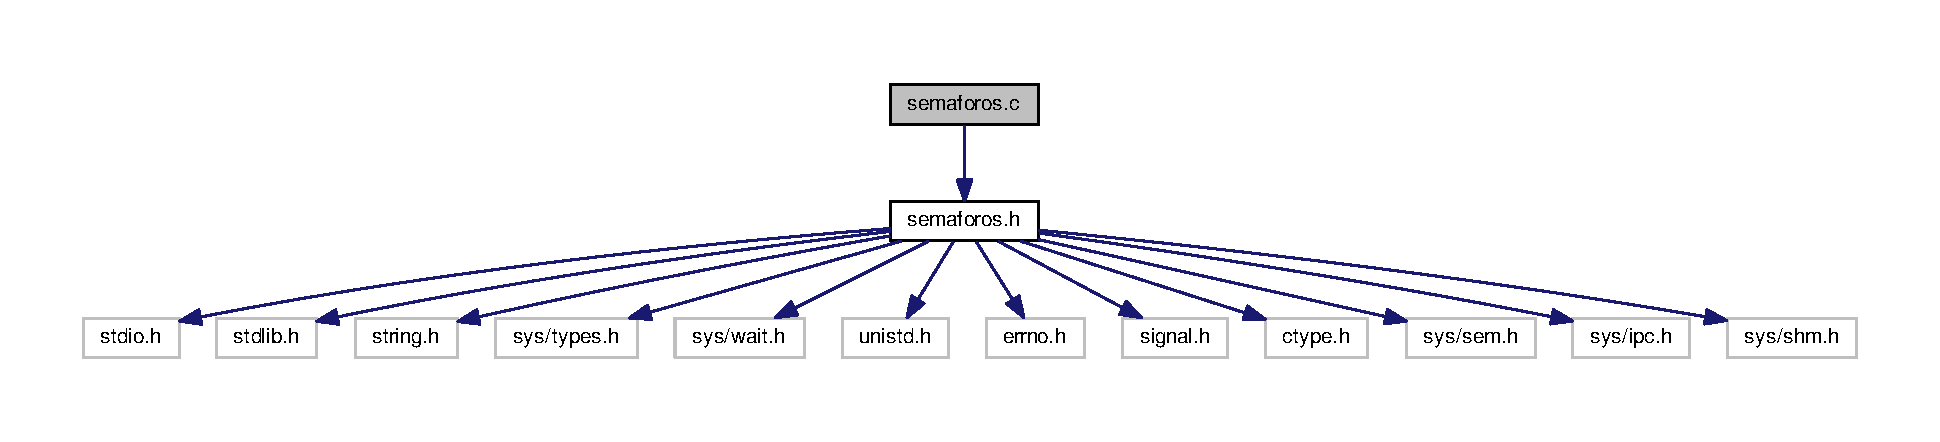
\includegraphics[width=350pt]{semaforos_8c__incl}
\end{center}
\end{figure}
\subsection*{Functions}
\begin{DoxyCompactItemize}
\item 
int \hyperlink{semaforos_8c_a4af104b0ed37e6ae0289a1059bc6e990}{Inicializar\+\_\+\+Semaforo} (int semid, unsigned short $\ast$array)
\begin{DoxyCompactList}\small\item\em funcion inicializadora de semaforos. Su funcionalidad es inicializar los semaforos indicados. \end{DoxyCompactList}\item 
int \hyperlink{semaforos_8c_a731339337960a681efa435a10f12c312}{Borrar\+\_\+\+Semaforo} (int semid)
\begin{DoxyCompactList}\small\item\em funcion que borra semaforos. Su funcionalidad es borrar el semaforo indicado. \end{DoxyCompactList}\item 
int \hyperlink{semaforos_8c_a16b16dd895b5f4cbe48f1ac8977e8b35}{Crear\+\_\+\+Semaforo} (key\+\_\+t key, int size, int $\ast$semid)
\begin{DoxyCompactList}\small\item\em funcion creadora de semaforos. Su funcionalidad es crear un semaforo con la clave y tamaño indicados. \end{DoxyCompactList}\item 
int \hyperlink{semaforos_8c_a883244cd3b83c42cda23687da1b63369}{Down\+\_\+\+Semaforo} (int id, int num\+\_\+sem, int undo)
\begin{DoxyCompactList}\small\item\em funcion que decrementa un semaforo. Su funcionalidad es bajar o decrementar el semaforo indicado. \end{DoxyCompactList}\item 
int \hyperlink{semaforos_8c_ab375ebfc38acbdced46e062a689d5fad}{Down\+Multiple\+\_\+\+Semaforo} (int id, int size, int undo, int $\ast$active)
\begin{DoxyCompactList}\small\item\em funcion que decrementa varios semaforos. Su funcionalidad es bajar o decrementar todos los semaforos indicados. \end{DoxyCompactList}\item 
int \hyperlink{semaforos_8c_a2d5e735aecee4f493898b3d4ebab1a10}{Up\+\_\+\+Semaforo} (int id, int num\+\_\+sem, int undo)
\begin{DoxyCompactList}\small\item\em funcion que incrementa un semaforo. Su funcionalidad es subir o incrementar el semaforo indicado. \end{DoxyCompactList}\item 
int \hyperlink{semaforos_8c_a943759695f018d64a94b8a2c49308092}{Up\+Multiple\+\_\+\+Semaforo} (int id, int size, int undo, int $\ast$active)
\begin{DoxyCompactList}\small\item\em funcion que incrementa varios semaforos. Su funcionalidad es subir o incrementar todos los semaforos indicados. \end{DoxyCompactList}\end{DoxyCompactItemize}


\subsection{Detailed Description}
Ejercicio9. 

Utilidades de manejo de semaforos.

Este ejercicio comprueba la librería de semaforos mientras ayuda didacticamente

\begin{DoxyAuthor}{Author}
Alejandro Santorum \& David Cabornero (G2202-\/\+Pareja7) 
\end{DoxyAuthor}
\begin{DoxyVersion}{Version}
1.\+0 
\end{DoxyVersion}
\begin{DoxyDate}{Date}
06-\/04-\/2018
\end{DoxyDate}
Este modulo contiene la implementacion de las funciones de manejo de semaforos.

\begin{DoxyAuthor}{Author}
Alejandro Santorum \& David Cabornero (G2202-\/\+Pareja7) 
\end{DoxyAuthor}
\begin{DoxyVersion}{Version}
1.\+0 
\end{DoxyVersion}
\begin{DoxyDate}{Date}
01-\/04-\/2018 
\end{DoxyDate}


\subsection{Function Documentation}
\index{semaforos.\+c@{semaforos.\+c}!Borrar\+\_\+\+Semaforo@{Borrar\+\_\+\+Semaforo}}
\index{Borrar\+\_\+\+Semaforo@{Borrar\+\_\+\+Semaforo}!semaforos.\+c@{semaforos.\+c}}
\subsubsection[{\texorpdfstring{Borrar\+\_\+\+Semaforo(int semid)}{Borrar_Semaforo(int semid)}}]{\setlength{\rightskip}{0pt plus 5cm}int Borrar\+\_\+\+Semaforo (
\begin{DoxyParamCaption}
\item[{int}]{semid}
\end{DoxyParamCaption}
)}\hypertarget{semaforos_8c_a731339337960a681efa435a10f12c312}{}\label{semaforos_8c_a731339337960a681efa435a10f12c312}


funcion que borra semaforos. Su funcionalidad es borrar el semaforo indicado. 


\begin{DoxyParams}{Parameters}
{\em semid} & -\/ identificador del semaforo \\
\hline
\end{DoxyParams}
\begin{DoxyReturn}{Returns}
OK si todo fue correcto, E\+R\+R\+OR en caso de error. 
\end{DoxyReturn}
\index{semaforos.\+c@{semaforos.\+c}!Crear\+\_\+\+Semaforo@{Crear\+\_\+\+Semaforo}}
\index{Crear\+\_\+\+Semaforo@{Crear\+\_\+\+Semaforo}!semaforos.\+c@{semaforos.\+c}}
\subsubsection[{\texorpdfstring{Crear\+\_\+\+Semaforo(key\+\_\+t key, int size, int $\ast$semid)}{Crear_Semaforo(key_t key, int size, int *semid)}}]{\setlength{\rightskip}{0pt plus 5cm}int Crear\+\_\+\+Semaforo (
\begin{DoxyParamCaption}
\item[{key\+\_\+t}]{key, }
\item[{int}]{size, }
\item[{int $\ast$}]{semid}
\end{DoxyParamCaption}
)}\hypertarget{semaforos_8c_a16b16dd895b5f4cbe48f1ac8977e8b35}{}\label{semaforos_8c_a16b16dd895b5f4cbe48f1ac8977e8b35}


funcion creadora de semaforos. Su funcionalidad es crear un semaforo con la clave y tamaño indicados. 


\begin{DoxyParams}{Parameters}
{\em key} & -\/ clave precompartida del semaforo \\
\hline
{\em size} & -\/ tamanio del semaforo. \\
\hline
{\em semid} & -\/ entero pasado por referencia para alojar el semid del semaforo creado \\
\hline
\end{DoxyParams}
\begin{DoxyReturn}{Returns}
int $\ast$semid -\/ identificador del semaforo. Int E\+R\+R\+OR en caso de error, 1 si el semaforo ya existia, 0 en caso de exito. 
\end{DoxyReturn}
\index{semaforos.\+c@{semaforos.\+c}!Down\+\_\+\+Semaforo@{Down\+\_\+\+Semaforo}}
\index{Down\+\_\+\+Semaforo@{Down\+\_\+\+Semaforo}!semaforos.\+c@{semaforos.\+c}}
\subsubsection[{\texorpdfstring{Down\+\_\+\+Semaforo(int id, int num\+\_\+sem, int undo)}{Down_Semaforo(int id, int num_sem, int undo)}}]{\setlength{\rightskip}{0pt plus 5cm}int Down\+\_\+\+Semaforo (
\begin{DoxyParamCaption}
\item[{int}]{id, }
\item[{int}]{num\+\_\+sem, }
\item[{int}]{undo}
\end{DoxyParamCaption}
)}\hypertarget{semaforos_8c_a883244cd3b83c42cda23687da1b63369}{}\label{semaforos_8c_a883244cd3b83c42cda23687da1b63369}


funcion que decrementa un semaforo. Su funcionalidad es bajar o decrementar el semaforo indicado. 


\begin{DoxyParams}{Parameters}
{\em id} & -\/ identificador del semaforo \\
\hline
{\em num\+\_\+sem} & -\/ semaforo dentro del array \\
\hline
{\em undo} & -\/ flag de modo persistente pese a finalizacion abrupta \\
\hline
\end{DoxyParams}
\begin{DoxyReturn}{Returns}
OK si todo fue correcto, E\+R\+R\+OR en caso de error. 
\end{DoxyReturn}
\index{semaforos.\+c@{semaforos.\+c}!Down\+Multiple\+\_\+\+Semaforo@{Down\+Multiple\+\_\+\+Semaforo}}
\index{Down\+Multiple\+\_\+\+Semaforo@{Down\+Multiple\+\_\+\+Semaforo}!semaforos.\+c@{semaforos.\+c}}
\subsubsection[{\texorpdfstring{Down\+Multiple\+\_\+\+Semaforo(int id, int size, int undo, int $\ast$active)}{DownMultiple_Semaforo(int id, int size, int undo, int *active)}}]{\setlength{\rightskip}{0pt plus 5cm}int Down\+Multiple\+\_\+\+Semaforo (
\begin{DoxyParamCaption}
\item[{int}]{id, }
\item[{int}]{size, }
\item[{int}]{undo, }
\item[{int $\ast$}]{active}
\end{DoxyParamCaption}
)}\hypertarget{semaforos_8c_ab375ebfc38acbdced46e062a689d5fad}{}\label{semaforos_8c_ab375ebfc38acbdced46e062a689d5fad}


funcion que decrementa varios semaforos. Su funcionalidad es bajar o decrementar todos los semaforos indicados. 


\begin{DoxyParams}{Parameters}
{\em id} & -\/ identificador del semaforo \\
\hline
{\em size} & -\/ tamanio del array de ids de los semaforos involucrados(active) \\
\hline
{\em undo} & -\/ flag de modo persistente pese a finalizacion abrupta \\
\hline
{\em active} & Semaforos involucrados. \\
\hline
\end{DoxyParams}
\begin{DoxyReturn}{Returns}
OK si todo fue correcto, E\+R\+R\+OR en caso de error. 
\end{DoxyReturn}
\index{semaforos.\+c@{semaforos.\+c}!Inicializar\+\_\+\+Semaforo@{Inicializar\+\_\+\+Semaforo}}
\index{Inicializar\+\_\+\+Semaforo@{Inicializar\+\_\+\+Semaforo}!semaforos.\+c@{semaforos.\+c}}
\subsubsection[{\texorpdfstring{Inicializar\+\_\+\+Semaforo(int semid, unsigned short $\ast$array)}{Inicializar_Semaforo(int semid, unsigned short *array)}}]{\setlength{\rightskip}{0pt plus 5cm}int Inicializar\+\_\+\+Semaforo (
\begin{DoxyParamCaption}
\item[{int}]{semid, }
\item[{unsigned short $\ast$}]{array}
\end{DoxyParamCaption}
)}\hypertarget{semaforos_8c_a4af104b0ed37e6ae0289a1059bc6e990}{}\label{semaforos_8c_a4af104b0ed37e6ae0289a1059bc6e990}


funcion inicializadora de semaforos. Su funcionalidad es inicializar los semaforos indicados. 


\begin{DoxyParams}{Parameters}
{\em semid} & -\/ identificador del semaforo \\
\hline
{\em array} & -\/ valores iniciales \\
\hline
\end{DoxyParams}
\begin{DoxyReturn}{Returns}
OK si todo fue correcto, E\+R\+R\+OR en caso de error. 
\end{DoxyReturn}
\index{semaforos.\+c@{semaforos.\+c}!Up\+\_\+\+Semaforo@{Up\+\_\+\+Semaforo}}
\index{Up\+\_\+\+Semaforo@{Up\+\_\+\+Semaforo}!semaforos.\+c@{semaforos.\+c}}
\subsubsection[{\texorpdfstring{Up\+\_\+\+Semaforo(int id, int num\+\_\+sem, int undo)}{Up_Semaforo(int id, int num_sem, int undo)}}]{\setlength{\rightskip}{0pt plus 5cm}int Up\+\_\+\+Semaforo (
\begin{DoxyParamCaption}
\item[{int}]{id, }
\item[{int}]{num\+\_\+sem, }
\item[{int}]{undo}
\end{DoxyParamCaption}
)}\hypertarget{semaforos_8c_a2d5e735aecee4f493898b3d4ebab1a10}{}\label{semaforos_8c_a2d5e735aecee4f493898b3d4ebab1a10}


funcion que incrementa un semaforo. Su funcionalidad es subir o incrementar el semaforo indicado. 


\begin{DoxyParams}{Parameters}
{\em id} & -\/ identificador del semaforo \\
\hline
{\em num\+\_\+sem} & -\/ semaforo dentro del array \\
\hline
{\em undo} & -\/ flag de modo persistente pese a finalizacion abrupta \\
\hline
\end{DoxyParams}
\begin{DoxyReturn}{Returns}
OK si todo fue correcto, E\+R\+R\+OR en caso de error. 
\end{DoxyReturn}
\index{semaforos.\+c@{semaforos.\+c}!Up\+Multiple\+\_\+\+Semaforo@{Up\+Multiple\+\_\+\+Semaforo}}
\index{Up\+Multiple\+\_\+\+Semaforo@{Up\+Multiple\+\_\+\+Semaforo}!semaforos.\+c@{semaforos.\+c}}
\subsubsection[{\texorpdfstring{Up\+Multiple\+\_\+\+Semaforo(int id, int size, int undo, int $\ast$active)}{UpMultiple_Semaforo(int id, int size, int undo, int *active)}}]{\setlength{\rightskip}{0pt plus 5cm}int Up\+Multiple\+\_\+\+Semaforo (
\begin{DoxyParamCaption}
\item[{int}]{id, }
\item[{int}]{size, }
\item[{int}]{undo, }
\item[{int $\ast$}]{active}
\end{DoxyParamCaption}
)}\hypertarget{semaforos_8c_a943759695f018d64a94b8a2c49308092}{}\label{semaforos_8c_a943759695f018d64a94b8a2c49308092}


funcion que incrementa varios semaforos. Su funcionalidad es subir o incrementar todos los semaforos indicados. 


\begin{DoxyParams}{Parameters}
{\em id} & -\/ identificador del semaforo \\
\hline
{\em size} & -\/ tamanio del array de ids de los semaforos involucrados(active) \\
\hline
{\em undo} & -\/ flag de modo persistente pese a finalizacion abrupta \\
\hline
{\em active} & Semaforos involucrados. \\
\hline
\end{DoxyParams}
\begin{DoxyReturn}{Returns}
OK si todo fue correcto, E\+R\+R\+OR en caso de error. 
\end{DoxyReturn}

\hypertarget{semaforos_8h}{}\section{semaforos.\+h File Reference}
\label{semaforos_8h}\index{semaforos.\+h@{semaforos.\+h}}


Utilidades de manejo de semaforos.  


{\ttfamily \#include $<$stdio.\+h$>$}\\*
{\ttfamily \#include $<$stdlib.\+h$>$}\\*
{\ttfamily \#include $<$string.\+h$>$}\\*
{\ttfamily \#include $<$sys/types.\+h$>$}\\*
{\ttfamily \#include $<$sys/wait.\+h$>$}\\*
{\ttfamily \#include $<$unistd.\+h$>$}\\*
{\ttfamily \#include $<$errno.\+h$>$}\\*
{\ttfamily \#include $<$signal.\+h$>$}\\*
{\ttfamily \#include $<$ctype.\+h$>$}\\*
{\ttfamily \#include $<$sys/sem.\+h$>$}\\*
{\ttfamily \#include $<$sys/ipc.\+h$>$}\\*
{\ttfamily \#include $<$sys/shm.\+h$>$}\\*
Include dependency graph for semaforos.\+h\+:
\nopagebreak
\begin{figure}[H]
\begin{center}
\leavevmode
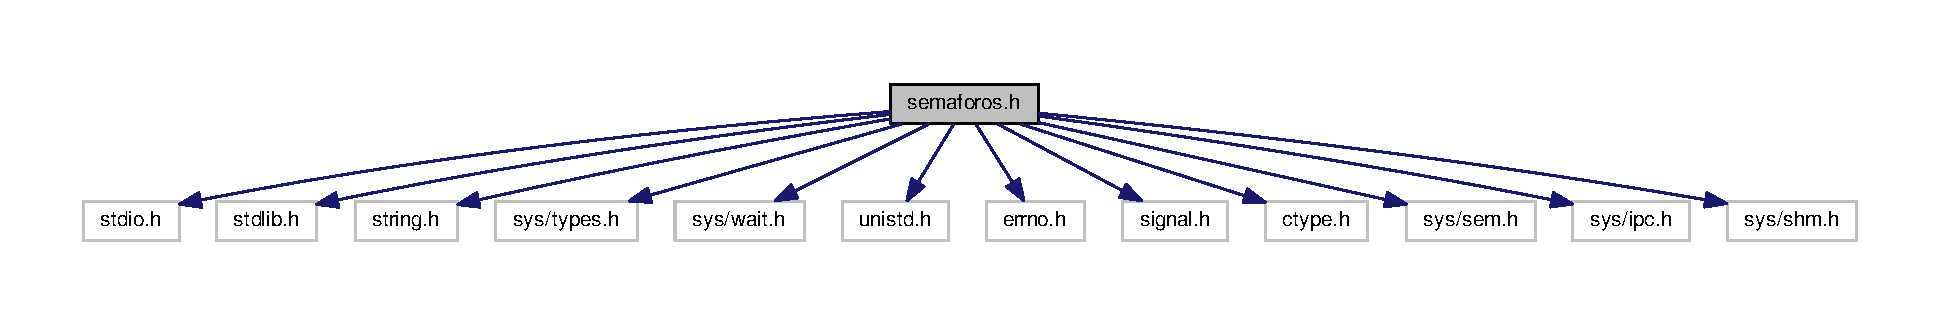
\includegraphics[width=350pt]{semaforos_8h__incl}
\end{center}
\end{figure}
This graph shows which files directly or indirectly include this file\+:
\nopagebreak
\begin{figure}[H]
\begin{center}
\leavevmode
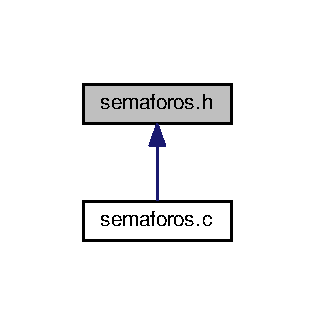
\includegraphics[width=151pt]{semaforos_8h__dep__incl}
\end{center}
\end{figure}
\subsection*{Macros}
\begin{DoxyCompactItemize}
\item 
\#define \hyperlink{semaforos_8h_a8fe83ac76edc595f6b98cd4a4127aed5}{E\+R\+R\+OR}~-\/1
\item 
\#define \hyperlink{semaforos_8h_aba51915c87d64af47fb1cc59348961c9}{OK}~0
\end{DoxyCompactItemize}
\subsection*{Functions}
\begin{DoxyCompactItemize}
\item 
int \hyperlink{semaforos_8h_a4af104b0ed37e6ae0289a1059bc6e990}{Inicializar\+\_\+\+Semaforo} (int semid, unsigned short $\ast$array)
\begin{DoxyCompactList}\small\item\em funcion inicializadora de semaforos. Su funcionalidad es inicializar los semaforos indicados. \end{DoxyCompactList}\item 
int \hyperlink{semaforos_8h_a731339337960a681efa435a10f12c312}{Borrar\+\_\+\+Semaforo} (int semid)
\begin{DoxyCompactList}\small\item\em funcion que borra semaforos. Su funcionalidad es borrar el semaforo indicado. \end{DoxyCompactList}\item 
int \hyperlink{semaforos_8h_a16b16dd895b5f4cbe48f1ac8977e8b35}{Crear\+\_\+\+Semaforo} (key\+\_\+t key, int size, int $\ast$semid)
\begin{DoxyCompactList}\small\item\em funcion creadora de semaforos. Su funcionalidad es crear un semaforo con la clave y tamaño indicados. \end{DoxyCompactList}\item 
int \hyperlink{semaforos_8h_a883244cd3b83c42cda23687da1b63369}{Down\+\_\+\+Semaforo} (int id, int num\+\_\+sem, int undo)
\begin{DoxyCompactList}\small\item\em funcion que decrementa un semaforo. Su funcionalidad es bajar o decrementar el semaforo indicado. \end{DoxyCompactList}\item 
int \hyperlink{semaforos_8h_ab375ebfc38acbdced46e062a689d5fad}{Down\+Multiple\+\_\+\+Semaforo} (int id, int size, int undo, int $\ast$active)
\begin{DoxyCompactList}\small\item\em funcion que decrementa varios semaforos. Su funcionalidad es bajar o decrementar todos los semaforos indicados. \end{DoxyCompactList}\item 
int \hyperlink{semaforos_8h_a2d5e735aecee4f493898b3d4ebab1a10}{Up\+\_\+\+Semaforo} (int id, int num\+\_\+sem, int undo)
\begin{DoxyCompactList}\small\item\em funcion que incrementa un semaforo. Su funcionalidad es subir o incrementar el semaforo indicado. \end{DoxyCompactList}\item 
int \hyperlink{semaforos_8h_a943759695f018d64a94b8a2c49308092}{Up\+Multiple\+\_\+\+Semaforo} (int id, int size, int undo, int $\ast$active)
\begin{DoxyCompactList}\small\item\em funcion que incrementa varios semaforos. Su funcionalidad es subir o incrementar todos los semaforos indicados. \end{DoxyCompactList}\end{DoxyCompactItemize}


\subsection{Detailed Description}
Utilidades de manejo de semaforos. 

Este modulo contiene los prototipos de las funciones de manejo de semaforos.

\begin{DoxyAuthor}{Author}
Alejandro Santorum \& David Cabornero (G2202-\/\+Pareja7) 
\end{DoxyAuthor}
\begin{DoxyVersion}{Version}
1.\+0 
\end{DoxyVersion}
\begin{DoxyDate}{Date}
01-\/04-\/2018 
\end{DoxyDate}


\subsection{Macro Definition Documentation}
\index{semaforos.\+h@{semaforos.\+h}!E\+R\+R\+OR@{E\+R\+R\+OR}}
\index{E\+R\+R\+OR@{E\+R\+R\+OR}!semaforos.\+h@{semaforos.\+h}}
\subsubsection[{\texorpdfstring{E\+R\+R\+OR}{ERROR}}]{\setlength{\rightskip}{0pt plus 5cm}\#define E\+R\+R\+OR~-\/1}\hypertarget{semaforos_8h_a8fe83ac76edc595f6b98cd4a4127aed5}{}\label{semaforos_8h_a8fe83ac76edc595f6b98cd4a4127aed5}
Constante con significado de operacion erronea \index{semaforos.\+h@{semaforos.\+h}!OK@{OK}}
\index{OK@{OK}!semaforos.\+h@{semaforos.\+h}}
\subsubsection[{\texorpdfstring{OK}{OK}}]{\setlength{\rightskip}{0pt plus 5cm}\#define OK~0}\hypertarget{semaforos_8h_aba51915c87d64af47fb1cc59348961c9}{}\label{semaforos_8h_aba51915c87d64af47fb1cc59348961c9}
Constante con significado de operacion exitosa 

\subsection{Function Documentation}
\index{semaforos.\+h@{semaforos.\+h}!Borrar\+\_\+\+Semaforo@{Borrar\+\_\+\+Semaforo}}
\index{Borrar\+\_\+\+Semaforo@{Borrar\+\_\+\+Semaforo}!semaforos.\+h@{semaforos.\+h}}
\subsubsection[{\texorpdfstring{Borrar\+\_\+\+Semaforo(int semid)}{Borrar_Semaforo(int semid)}}]{\setlength{\rightskip}{0pt plus 5cm}int Borrar\+\_\+\+Semaforo (
\begin{DoxyParamCaption}
\item[{int}]{semid}
\end{DoxyParamCaption}
)}\hypertarget{semaforos_8h_a731339337960a681efa435a10f12c312}{}\label{semaforos_8h_a731339337960a681efa435a10f12c312}


funcion que borra semaforos. Su funcionalidad es borrar el semaforo indicado. 


\begin{DoxyParams}{Parameters}
{\em semid} & -\/ identificador del semaforo \\
\hline
\end{DoxyParams}
\begin{DoxyReturn}{Returns}
OK si todo fue correcto, E\+R\+R\+OR en caso de error. 
\end{DoxyReturn}
\index{semaforos.\+h@{semaforos.\+h}!Crear\+\_\+\+Semaforo@{Crear\+\_\+\+Semaforo}}
\index{Crear\+\_\+\+Semaforo@{Crear\+\_\+\+Semaforo}!semaforos.\+h@{semaforos.\+h}}
\subsubsection[{\texorpdfstring{Crear\+\_\+\+Semaforo(key\+\_\+t key, int size, int $\ast$semid)}{Crear_Semaforo(key_t key, int size, int *semid)}}]{\setlength{\rightskip}{0pt plus 5cm}int Crear\+\_\+\+Semaforo (
\begin{DoxyParamCaption}
\item[{key\+\_\+t}]{key, }
\item[{int}]{size, }
\item[{int $\ast$}]{semid}
\end{DoxyParamCaption}
)}\hypertarget{semaforos_8h_a16b16dd895b5f4cbe48f1ac8977e8b35}{}\label{semaforos_8h_a16b16dd895b5f4cbe48f1ac8977e8b35}


funcion creadora de semaforos. Su funcionalidad es crear un semaforo con la clave y tamaño indicados. 


\begin{DoxyParams}{Parameters}
{\em key} & -\/ clave precompartida del semaforo \\
\hline
{\em size} & -\/ tamanio del semaforo. \\
\hline
{\em semid} & -\/ entero pasado por referencia para alojar el semid del semaforo creado \\
\hline
\end{DoxyParams}
\begin{DoxyReturn}{Returns}
int $\ast$semid -\/ identificador del semaforo. Int E\+R\+R\+OR en caso de error, 1 si el semaforo ya existia, 0 en caso de exito. 
\end{DoxyReturn}
\index{semaforos.\+h@{semaforos.\+h}!Down\+\_\+\+Semaforo@{Down\+\_\+\+Semaforo}}
\index{Down\+\_\+\+Semaforo@{Down\+\_\+\+Semaforo}!semaforos.\+h@{semaforos.\+h}}
\subsubsection[{\texorpdfstring{Down\+\_\+\+Semaforo(int id, int num\+\_\+sem, int undo)}{Down_Semaforo(int id, int num_sem, int undo)}}]{\setlength{\rightskip}{0pt plus 5cm}int Down\+\_\+\+Semaforo (
\begin{DoxyParamCaption}
\item[{int}]{id, }
\item[{int}]{num\+\_\+sem, }
\item[{int}]{undo}
\end{DoxyParamCaption}
)}\hypertarget{semaforos_8h_a883244cd3b83c42cda23687da1b63369}{}\label{semaforos_8h_a883244cd3b83c42cda23687da1b63369}


funcion que decrementa un semaforo. Su funcionalidad es bajar o decrementar el semaforo indicado. 


\begin{DoxyParams}{Parameters}
{\em id} & -\/ identificador del semaforo \\
\hline
{\em num\+\_\+sem} & -\/ semaforo dentro del array \\
\hline
{\em undo} & -\/ flag de modo persistente pese a finalizacion abrupta \\
\hline
\end{DoxyParams}
\begin{DoxyReturn}{Returns}
OK si todo fue correcto, E\+R\+R\+OR en caso de error. 
\end{DoxyReturn}
\index{semaforos.\+h@{semaforos.\+h}!Down\+Multiple\+\_\+\+Semaforo@{Down\+Multiple\+\_\+\+Semaforo}}
\index{Down\+Multiple\+\_\+\+Semaforo@{Down\+Multiple\+\_\+\+Semaforo}!semaforos.\+h@{semaforos.\+h}}
\subsubsection[{\texorpdfstring{Down\+Multiple\+\_\+\+Semaforo(int id, int size, int undo, int $\ast$active)}{DownMultiple_Semaforo(int id, int size, int undo, int *active)}}]{\setlength{\rightskip}{0pt plus 5cm}int Down\+Multiple\+\_\+\+Semaforo (
\begin{DoxyParamCaption}
\item[{int}]{id, }
\item[{int}]{size, }
\item[{int}]{undo, }
\item[{int $\ast$}]{active}
\end{DoxyParamCaption}
)}\hypertarget{semaforos_8h_ab375ebfc38acbdced46e062a689d5fad}{}\label{semaforos_8h_ab375ebfc38acbdced46e062a689d5fad}


funcion que decrementa varios semaforos. Su funcionalidad es bajar o decrementar todos los semaforos indicados. 


\begin{DoxyParams}{Parameters}
{\em id} & -\/ identificador del semaforo \\
\hline
{\em size} & -\/ tamanio del array de ids de los semaforos involucrados(active) \\
\hline
{\em undo} & -\/ flag de modo persistente pese a finalizacion abrupta \\
\hline
{\em active} & Semaforos involucrados. \\
\hline
\end{DoxyParams}
\begin{DoxyReturn}{Returns}
OK si todo fue correcto, E\+R\+R\+OR en caso de error. 
\end{DoxyReturn}
\index{semaforos.\+h@{semaforos.\+h}!Inicializar\+\_\+\+Semaforo@{Inicializar\+\_\+\+Semaforo}}
\index{Inicializar\+\_\+\+Semaforo@{Inicializar\+\_\+\+Semaforo}!semaforos.\+h@{semaforos.\+h}}
\subsubsection[{\texorpdfstring{Inicializar\+\_\+\+Semaforo(int semid, unsigned short $\ast$array)}{Inicializar_Semaforo(int semid, unsigned short *array)}}]{\setlength{\rightskip}{0pt plus 5cm}int Inicializar\+\_\+\+Semaforo (
\begin{DoxyParamCaption}
\item[{int}]{semid, }
\item[{unsigned short $\ast$}]{array}
\end{DoxyParamCaption}
)}\hypertarget{semaforos_8h_a4af104b0ed37e6ae0289a1059bc6e990}{}\label{semaforos_8h_a4af104b0ed37e6ae0289a1059bc6e990}


funcion inicializadora de semaforos. Su funcionalidad es inicializar los semaforos indicados. 


\begin{DoxyParams}{Parameters}
{\em semid} & -\/ identificador del semaforo \\
\hline
{\em array} & -\/ valores iniciales \\
\hline
\end{DoxyParams}
\begin{DoxyReturn}{Returns}
OK si todo fue correcto, E\+R\+R\+OR en caso de error. 
\end{DoxyReturn}
\index{semaforos.\+h@{semaforos.\+h}!Up\+\_\+\+Semaforo@{Up\+\_\+\+Semaforo}}
\index{Up\+\_\+\+Semaforo@{Up\+\_\+\+Semaforo}!semaforos.\+h@{semaforos.\+h}}
\subsubsection[{\texorpdfstring{Up\+\_\+\+Semaforo(int id, int num\+\_\+sem, int undo)}{Up_Semaforo(int id, int num_sem, int undo)}}]{\setlength{\rightskip}{0pt plus 5cm}int Up\+\_\+\+Semaforo (
\begin{DoxyParamCaption}
\item[{int}]{id, }
\item[{int}]{num\+\_\+sem, }
\item[{int}]{undo}
\end{DoxyParamCaption}
)}\hypertarget{semaforos_8h_a2d5e735aecee4f493898b3d4ebab1a10}{}\label{semaforos_8h_a2d5e735aecee4f493898b3d4ebab1a10}


funcion que incrementa un semaforo. Su funcionalidad es subir o incrementar el semaforo indicado. 


\begin{DoxyParams}{Parameters}
{\em id} & -\/ identificador del semaforo \\
\hline
{\em num\+\_\+sem} & -\/ semaforo dentro del array \\
\hline
{\em undo} & -\/ flag de modo persistente pese a finalizacion abrupta \\
\hline
\end{DoxyParams}
\begin{DoxyReturn}{Returns}
OK si todo fue correcto, E\+R\+R\+OR en caso de error. 
\end{DoxyReturn}
\index{semaforos.\+h@{semaforos.\+h}!Up\+Multiple\+\_\+\+Semaforo@{Up\+Multiple\+\_\+\+Semaforo}}
\index{Up\+Multiple\+\_\+\+Semaforo@{Up\+Multiple\+\_\+\+Semaforo}!semaforos.\+h@{semaforos.\+h}}
\subsubsection[{\texorpdfstring{Up\+Multiple\+\_\+\+Semaforo(int id, int size, int undo, int $\ast$active)}{UpMultiple_Semaforo(int id, int size, int undo, int *active)}}]{\setlength{\rightskip}{0pt plus 5cm}int Up\+Multiple\+\_\+\+Semaforo (
\begin{DoxyParamCaption}
\item[{int}]{id, }
\item[{int}]{size, }
\item[{int}]{undo, }
\item[{int $\ast$}]{active}
\end{DoxyParamCaption}
)}\hypertarget{semaforos_8h_a943759695f018d64a94b8a2c49308092}{}\label{semaforos_8h_a943759695f018d64a94b8a2c49308092}


funcion que incrementa varios semaforos. Su funcionalidad es subir o incrementar todos los semaforos indicados. 


\begin{DoxyParams}{Parameters}
{\em id} & -\/ identificador del semaforo \\
\hline
{\em size} & -\/ tamanio del array de ids de los semaforos involucrados(active) \\
\hline
{\em undo} & -\/ flag de modo persistente pese a finalizacion abrupta \\
\hline
{\em active} & Semaforos involucrados. \\
\hline
\end{DoxyParams}
\begin{DoxyReturn}{Returns}
OK si todo fue correcto, E\+R\+R\+OR en caso de error. 
\end{DoxyReturn}

%--- End generated contents ---

% Index
\backmatter
\newpage
\phantomsection
\clearemptydoublepage
\addcontentsline{toc}{chapter}{Index}
\printindex

\end{document}
